% =====================================================================
% Supplementary material -- Reformer digital twin
% Overleaf: add this as a second document in the same project (supplementary.tex)
% and compile it separately. Figures go in the same figures/ folder.
% =====================================================================
\documentclass[final,3p,times]{elsarticle}

\usepackage{amsmath,amssymb}
\usepackage{graphicx}
\usepackage{booktabs}
\usepackage{xcolor}
\usepackage[hidelinks]{hyperref}

\graphicspath{{figures/}}
\newcommand{\todo}[1]{\textcolor{red}{[TODO: #1]}}
\newcommand{\ce}[1]{\mathrm{#1}}

\renewcommand{\thesection}{S\arabic{section}}
\renewcommand{\thetable}{S\arabic{table}}
\renewcommand{\thefigure}{S\arabic{figure}}

\journal{International Journal of Hydrogen Energy}

\begin{document}

\begin{frontmatter}
\title{Supplementary material for: A physics-informed digital twin for tube-life-aware operation of industrial steam methane reformers under uncertainty}
\author[su]{Izbassar Orynbassar\corref{cor1}}
\ead{iorynbas@syr.edu}
\author[au]{Madina Sissenbay}
\cortext[cor1]{Corresponding author.}
\affiliation[su]{organization={School of Information Studies, Syracuse University},
  city={Syracuse}, state={NY}, country={USA}}
\affiliation[au]{organization={Institute of Petrochemical Engineering and Ecology named after N.K. Nadirov,
  Safi Utebayev Atyrau University of Oil and Gas},
  city={Atyrau}, country={Kazakhstan}}
\end{frontmatter}

% =====================================================================
\section{Model implementation detail}
\label{sec:modeldetail}

\paragraph{Effectiveness factors} Intraparticle diffusion limitation is severe in reformer catalysts. Rather than solving the pellet problem, the constant effectiveness factors adopted by Latham et al.~\cite{latham2011} following Wesenberg and Svendsen~\cite{wesenberg2007} are used: $\eta_j = 0.1$ along the tube and $0.05$ in the first tube section (10\,\% of the length here), where the feed contains little hydrogen and the rate expressions are stiff.

\paragraph{Higher alkanes at the inlet} Higher alkanes in the feed (C$_2$--C$_5$) are converted at the inlet by the overall rule used by Latham~\cite{latham2011},
\begin{equation}
\ce{C_kH_{2k+2}} + \tfrac{k-1}{3}\,\ce{H_2O} \rightarrow \tfrac{k-1}{3}\,\ce{CO} + \tfrac{2k+1}{3}\,\ce{CH_4},
\label{eq:alkane}
\end{equation}
whose enthalpy is small because the endothermic reforming and the exothermic hydrogenolysis nearly cancel.

\paragraph{Equilibrium constants and the hydrogen floor} The equilibrium constants computed from Gibbs energies of formation agree with the common empirical expressions within 7\,\% between 800 and 1100~K. A floor of $10^{-6}$~bar on $p_{\ce{H_2}}$ avoids the singularity of the rate expressions at a hydrogen-free inlet.

\paragraph{Heat-release profile and furnace-side convection} The heat-release density $r(z)$ of the long-furnace model is a downward-opening parabola that vanishes at $z = L_q L$, releases the fraction $\alpha_{\mathrm{top}}$ of the heat in the top fifteenth of the furnace height and integrates to $(1 - f_{\mathrm{loss}})\,Q_{\mathrm{comb}}$, with $f_{\mathrm{loss}} = 0.02$ for casing losses; this is the continuous form of the sectional heat-release profile of Latham~\cite{latham2011}. The furnace-side convective coefficient $h_c$ is taken from the Dittus--Boelter correlation on the flue-gas flow area, scaled by the factor $f_{\mathrm{ctube}} = 0.38$ fitted by Latham et al.~\cite{latham2011}; at furnace-gas temperatures the convective term is a minor correction to the radiative flux. The combustion heat $Q_{\mathrm{comb}}$ and the flue-gas flow and composition follow from the lower heating value and complete combustion of the fuel gas and pressure-swing-adsorption off-gas with the specified excess air.

\paragraph{Coupled solution} The outer-wall temperature at each height is found by a bracketed root search on the flux balance, evaluated inside the right-hand side of the ODE system, so that the furnace and tube equations are integrated together in a single downward sweep.

\paragraph{Thermal stress across the tube wall} The elastic thermal stress from the radial temperature gradient, $E\alpha\Delta T_{\mathrm{wall}}/[2(1-\nu)]$, is about 45~MPa for the 20--30~K wall drop of the calibrated tube ($E \approx 150$~GPa, $\alpha \approx 18 \times 10^{-6}$~K$^{-1}$ at 900~$^\circ$C, $\nu = 0.3$), several times the 12~MPa hoop stress.

\paragraph{Thermal time constants} The thermal time constant of the tube wall, $\rho c\,t^2/\lambda$, is of the order of one minute; that of the refractory lining is of the order of a day.

\paragraph{Calibration procedure} The nine residuals per plant case are the outlet temperature, the outlet pressure, the outlet wet composition, the flue-gas outlet temperature and the two wall temperatures. The trust-region-reflective algorithm with bounds is started from a Latin-hypercube set of initial points to guard against local minima, and the parameter covariance is obtained from the Jacobian at the optimum with $t$-based 95\,\% intervals.

% =====================================================================
\section{Operating space and campaign design}
\label{sec:ranges}

\begin{table}[h]
\centering\footnotesize
\caption{Operating space sampled in the design, sensitivity, surrogate and optimisation campaigns. The base column is the calibrated Plant~A state. Ranges are motivated by industrial practice and by the operating points of the sources used for verification and calibration.}
\label{tab:ranges}
\begin{tabular}{llccc p{5.6cm}}
\toprule
Variable & Unit & Min & Max & Base & Basis \\
\midrule
steam-to-carbon ratio & -- & 2.5 & 4.0 & 2.89 & carbon-formation limit on Ni catalyst below about 2.5; upper value typical of hydrogen plants; 2.7--3.0 in the reference plant~\cite{latham2011}, 3.36 in~\cite{xu1989b} \\
feed per tube & fraction of base & 0.60 & 1.10 & 1.00 & industrial turndown of about 50--60\,\%; 110\,\% short-term overload \\
specific firing $Q_{\mathrm{comb}}$/feed & fraction of base & 0.85 & 1.15 & 1.00 & burner control range around the plant value \\
inlet temperature & K & 800 & 900 & 884.5 & 884.5~K in the reference plant, 793~K in~\cite{xu1989b}; cracking in the preheat coil above about 920~K \\
inlet pressure & bar & 25 & 33 & 30.1 & industrial range 20--40~bar; 28--30~bar in the reference plant, 29~bar in~\cite{xu1989b} \\
catalyst activity & -- & 0.10 & 0.30 & 0.20 & 0.20 fitted to the reference plant for a mid-campaign catalyst~\cite{latham2011}; fresh higher, end-of-campaign lower \\
excess air & \% & 5 & 25 & 21.6 & industrial reformer furnaces 5--20\,\%; upper value extended so that the calibrated base lies inside the sampled space \\
\bottomrule
\end{tabular}
\end{table}

The campaigns evaluated on this space are: an open-loop Latin-hypercube design of 2000 points (surrogate training); a Saltelli design of 4096 points for the Sobol indices and as an independent surrogate test set; a closed-loop $15 \times 15$ grid in steam-to-carbon ratio and load at constant outlet temperature (Fig.~5 of the main text); twenty scenario-years of 8760 hourly states; an NSGA-II run of 200 individuals over 300 generations; and a scrambled Sobol Monte Carlo design of 2048 samples propagated through the physics model at eight operating points, with 1024 further samples per uncertainty group for the variance decomposition. All designs use seed~0. The complete pipeline runs in 35~minutes on a ten-core laptop.

\begin{table}[h]
\centering\footnotesize
\caption{Definitions of the six annual scenarios of Section~2.7 of the main text. Each is an 8760-hour hourly history evaluated under one of the two control modes.}
\label{tab:scendef}
\begin{tabular}{ll p{9.2cm}}
\toprule
Scenario & Control mode & Definition \\
\midrule
S1 steady base & either & constant operation at the calibrated Plant~A state \\
S2 daily load-following & either & full load 06--22~h, 70\,\% at night, ramps of 0.10 per hour \\
S3 renewable-following & either & bounded Ornstein--Uhlenbeck load process between 0.60 and 1.10 with mean 0.85 \\
S4 over-firing events & either & 24 events per year of $+10$\,\% firing for 2~h; six events of $+25$\,\% for 1~h; a flame-impingement proxy adding 40~K to the hot spot for 24~h per year \\
S5 catalyst ageing & both, separately & activity falling linearly from 0.30 to 0.10 over four years \\
S6 steam-to-carbon & either & steady operation at steam-to-carbon 2.5 and at 3.5 \\
\bottomrule
\end{tabular}
\end{table}

\begin{table}[h]
\centering\footnotesize
\caption{Uncertainty groups propagated in RQ4 and the distribution assigned to each input.}
\label{tab:uqgroups}
\begin{tabular}{ll p{8.6cm}}
\toprule
Group & Inputs & Distribution \\
\midrule
kinetics & $k_1$--$k_3$, $K_{\mathrm{CO}}$, $K_{\mathrm{H_2}}$, $K_{\mathrm{CH_4}}$, $K_{\mathrm{H_2O}}$ & normal, from the 95\,\% intervals reported by Xu and Froment~\cite{xu1989a} \\
 & effectiveness factors & log-uniform factor 0.5--2 \\
 & catalyst activity & uniform $\pm 0.03$ \\
heat transfer & $F_{\mathrm{gt}}$, $L_q$, $f_{\mathrm{htg}}$ & multivariate normal with the joint covariance of the calibration \\
creep & scatter on $\log_{10} t_r$ & normal, 0.181 decades, from the data-sheet band \\
 & Larson--Miller constant $C$ & uniform within $\pm 1$ of 18.6 \\
 & wall thickness & uniform 12--18~mm \\
 & tube conductivity & uniform $\pm 15$\,\% \\
measurement & hot-spot temperature offset & uniform $\pm 10$~K on the pyrometer reference \\
\bottomrule
\end{tabular}
\end{table}

\paragraph{Basis of the hot-spot temperature limit} The optimisation constrains the hot-spot temperature to 1193~K (920~$^\circ$C), close to the 925~$^\circ$C design tube-metal temperature used by Yeh~\cite{yeh2021} for an HP-Nb tube and 46~K above the calibrated base hot spot.

\paragraph{Enthalpy basis of the steam credit} The steam duty charged at $\alpha < 1$ is the heat needed to raise the process steam from liquid water at 25~$^\circ$C to vapour at the inlet temperature, plus the heat needed to preheat the dry feed to the inlet temperature.

\paragraph{The flame-length variant is a bound} The structural variant $L_q\,\mathrm{load}^{0.5}$ of the uncertainty analysis is a bound, not an expectation: the length of a turbulent jet diffusion flame is nearly independent of the jet velocity for a given burner~\cite{hawthorne1949}, so that reducing the fuel flow through all burners leaves the release profile essentially unchanged (the nominal case), whereas taking burner rows out of service at turndown, a common practice, redistributes the heat release in a way that the published data cannot constrain.

% =====================================================================
\section{Surrogate performance}
\label{sec:surrogate}

The eight surrogate targets are the hot-spot temperature $T_{\mathrm{wo,max}}$ and its axial position, the outlet temperature and pressure, the dry methane slip, the net hydrogen per tube, the absorbed duty and $\log_{10} t_r$ at the hot spot. Three model families are compared with scikit-learn~\cite{sklearn}: Gaussian-process regression with a Mat\'ern~5/2 kernel on a 1000-point subset, histogram gradient boosting and a multilayer perceptron. Each family is fitted twice, once on the seven operating inputs alone and once with two physics-derived features added: the equilibrium methane conversion at outlet conditions and the specific duty.
\begin{table}[h]
\centering\footnotesize
\caption{Best surrogate per target ($N_{\mathrm{train}} = 2000$ Latin-hypercube points, $N_{\mathrm{test}} = 4096$ Saltelli points): model family and feature set, test $R^2$ and RMSE, five-fold cross-validated RMSE, and empirical coverage (PICP) and mean width (MPIW) of the nominal 90\,\% CV+ conformal interval. ``physics'' denotes the feature set augmented with the equilibrium methane conversion and the specific duty.}
\label{tab:surrogate}
\begin{tabular}{llccccc}
\toprule
Target & Unit & Model & $R^2$ & RMSE & CV RMSE & PICP$_{90}$ / MPIW$_{90}$ \\
\midrule
$T_{\mathrm{wo,max}}$ & K & GP, physics & 1.000 & 0.113 & 0.133 & 0.957 / 0.25 \\
$z/L$ at $T_{\mathrm{wo,max}}$ & -- & MLP, base & 0.644 & 0.0319 & 0.0522 & 0.971 / 0.050 \\
$T_{\mathrm{out}}$ & K & GP, physics & 1.000 & 0.0182 & 0.0254 & 0.940 / 0.061 \\
$p_{\mathrm{out}}$ & bar & GP, base & 1.000 & $2.87\times10^{-4}$ & $5.63\times10^{-4}$ & 0.961 / $1.0\times10^{-3}$ \\
CH$_4$ slip (dry) & \% & GP, physics & 1.000 & $1.25\times10^{-3}$ & $1.42\times10^{-3}$ & 0.953 / $4.0\times10^{-3}$ \\
H$_2$ per tube & kmol\,h$^{-1}$ & GP, base & 1.000 & $8.47\times10^{-4}$ & $1.16\times10^{-3}$ & 0.946 / $2.9\times10^{-3}$ \\
absorbed duty & W & GP, base & 1.000 & $3.9\times10^{3}$ & $4.14\times10^{3}$ & 0.949 / $1.2\times10^{4}$ \\
$\log_{10} t_r$ at hot spot & -- & GP, base & 0.9999 & $5.66\times10^{-3}$ & $5.97\times10^{-3}$ & 0.959 / 0.011 \\
\bottomrule
\end{tabular}
\end{table}

\begin{figure}[h]
\centering
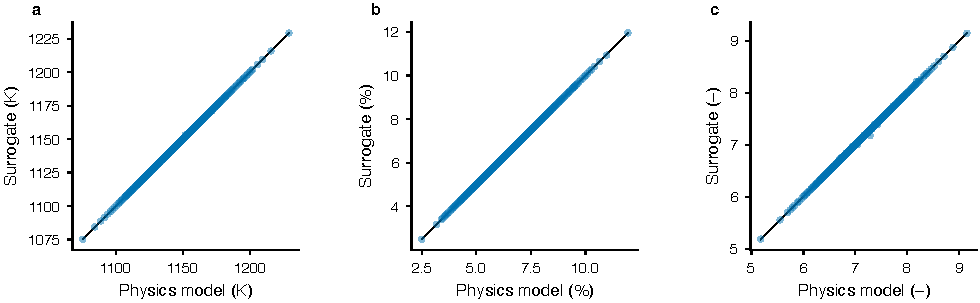
\includegraphics[width=\textwidth]{fig09_surrogate_parity}
\caption{Parity of the selected surrogates against the physics model on the independent Saltelli test set for (a) the hot-spot temperature, (b) dry methane slip and (c) $\log_{10} t_r$ at the hot spot, with nominal 90\,\% CV+ conformal intervals.}
\label{fig:surrogate}
\end{figure}


The Gaussian process dominates the other families by one to two orders of magnitude in RMSE on every continuous target, which is expected because the physics model is smooth and deterministic and the surrogate is effectively interpolating it; histogram gradient boosting is the weakest, with an RMSE of about 3~K on the hot-spot temperature. The location of the hot spot is the only target that is not learnable: it is bimodal, sitting near $z/L = 0.43$ for most inputs and moving to the outlet plateau for others, and all three families give $R^2$ below 0.65. It is reported for completeness and is not used in the life calculation, which requires only the maximum. Prediction takes 38~$\mu$s per point against 0.25~s for the physics model.

% =====================================================================
\section{Digitisation of the verification curves}
\label{sec:digitisation}

Figure~3 of Xu and Froment~\cite{xu1989b} reports six axial profiles for one industrial reformer tube on three vertical axes: methane and CO$_2$ conversion on the left axis, total pressure in bar and the process-gas, inner-wall and outer-wall temperatures in kelvin on two right axes. The figure was digitised with WebPlotDigitizer (version 5) from a 600~dpi scan of the printed page. Three independent axis calibrations were defined on the same image, one per vertical axis, each anchored on two gridline labels of the horizontal axis (0 and 10~m) and two labels of the corresponding vertical axis (0 and 0.8 for conversion, 24 and 29~bar for pressure, 800 and 1150~K for temperature). Points were placed manually along each curve at intervals of roughly 0.05~m of the tube length, with additional points concentrated at the discontinuity at the end of the heated length ($z = 11.12$~m), giving 118--261 points per curve.

The left axis of the original figure is labelled $x/(1+\zeta)$, where $\zeta = 0.056$ is the CO$_2$/CH$_4$ molar ratio of the feed; the digitised ordinates of the two conversion curves are therefore multiplied by $1+\zeta$ to obtain conversions referred to the equivalent methane feed. The residual uncertainty of the digitisation, estimated from the spread of repeated point placements on the gridlines, is about 2~K in temperature, 0.03~bar in pressure and 0.005 in conversion, which is small compared with the model residuals reported in the main text. The digitised curves, the axis calibrations and a tidy merged file with provenance metadata are in \texttt{data/literature\_validation/digitized/} of the repository.

Two features of the digitised data are recorded but not corrected. The digitised process-gas temperature begins at 764~K whereas Table~2 of the same paper states an inlet temperature of 793~K, so all temperature comparisons in the main text exclude $z < 0.3$~m. Both conversion curves begin at about 0.057 rather than at zero; this value lies between the inlet conversion implied by the higher-alkane rule used here (0.018) and the value obtained if all C$_2$--C$_5$ carbon is converted to CO at the inlet (0.091), and the conversion increment $x(z) - x(0.5~\mathrm{m})$ is therefore used as the primary comparison metric. The offset is consistent with a steep initial rise that the printed figure does not resolve, and it accounts for the residual of about 0.04 in absolute conversion reported in the main text.

% =====================================================================
\section{Verification and calibration detail}
\label{sec:verifdetail}

\begin{table}[t]
\centering\footnotesize
\caption{Verification of the tube model against the digitised Fig.~3 of Xu and Froment~\cite{xu1989b}: RMSE of methane conversion $x_{\ce{CH_4}}$, of the conversion increment $x(z) - x(0.5~\mathrm{m})$, of the process-gas and inner-wall temperatures ($z \geq 0.3$~m) and of pressure. Bed voidage 0.526 and equivalent particle diameter 9.44~mm fitted to the pressure profile.}
\label{tab:xf}
\begin{tabular}{lccccc}
\toprule
Configuration & RMSE $x_{\ce{CH_4}}$ & RMSE $\Delta x$ & RMSE $T_g$ (K) & RMSE $T_{\mathrm{wi}}$ (K) & RMSE $p$ (bar) \\
\midrule
Leva--Grummer, $f_{\mathrm{htg}}=1$, $\eta = 0.1$ & 0.160 & -- & 75.4 & 37.5 & 0.04 \\
matched $\alpha_i = 348$~W\,m$^{-2}$\,K$^{-1}$, $\eta = 0.1$ & 0.037 & 0.020 & 13.7 & 16.7 & 0.25 \\
matched $\alpha_i$, $\eta = 0.05/0.1$ (adopted) & 0.039 & 0.015 & 14.0 & 16.7 & 0.25 \\
matched $\alpha_i(z)$ profile, $\eta = 0.05/0.1$ & 0.046 & 0.017 & 17.6 & 16.9 & 0.26 \\
\bottomrule
\multicolumn{6}{l}{\scriptsize Back-calculated $\alpha_i$: median 348, interquartile range 313--363~W\,m$^{-2}$\,K$^{-1}$ over 0.5--11~m.}
\end{tabular}
\end{table}

\begin{table}[t]
\centering\footnotesize
\caption{Calibrated furnace and heat-transfer parameters on Plants~A, B and C2 with 95\,\% $t$-intervals from the Jacobian covariance. The four-parameter fit has $\alpha_{\mathrm{top}}$ at its bound with $r(L_q, \alpha_{\mathrm{top}}) = 0.985$; the adopted fit fixes $\alpha_{\mathrm{top}} = 0.182$.}
\label{tab:params}
\begin{tabular}{llccc}
\toprule
Fit & Parameter & Value & 95\,\% interval & s.e. \\
\midrule
four parameters & $F_{\mathrm{gt}}$ & 0.316 & [0.286, 0.346] & 0.014 \\
 & $L_q$ & 0.497 & [0.329, 0.665] & 0.081 \\
 & $\alpha_{\mathrm{top}}$ & 0.400 & [$-0.261$, 1.061] & 0.32 \\
 & $f_{\mathrm{htg}}$ & 1.74 & [1.427, 2.051] & 0.15 \\
 & $\chi^2$ / dof & 30.5 / 23 & reduced 1.32 & \\
\midrule
$\alpha_{\mathrm{top}}$ fixed (adopted) & $F_{\mathrm{gt}}$ & 0.323 & [0.309, 0.338] & 0.0072 \\
 & $L_q$ & 0.456 & [0.434, 0.478] & 0.011 \\
 & $f_{\mathrm{htg}}$ & 1.83 & [1.617, 2.052] & 0.11 \\
 & $\chi^2$ / dof & 34.9 / 24 & reduced 1.46 & \\
\bottomrule
\end{tabular}
\end{table}

The pressure RMSE of the verification runs rises from 0.04~bar with the Leva--Grummer configuration to 0.25~bar with the matched film coefficient. This is not a deterioration of the friction model, which is unchanged between the two: the bed voidage and equivalent particle diameter were fitted to the pressure profile under the hotter Leva--Grummer gas, and the cooler gas of the matched run has a higher density and a lower velocity at the same mass flow.

% =====================================================================
\section{Steam-credit sweep}
\label{sec:steamcredit}

\begin{table}[h]
\centering\footnotesize
\caption{Steam-credit sweep of the iso-production (H$_2$ = base $\pm 1$\,\%) life--fuel front. $\alpha = 1$ counts firebox fuel only; $\alpha = 0$ charges steam raising and feed preheat in full. All rows are physics-verified.}
\label{tab:steam}
\begin{tabular}{llcccccccc}
\toprule
$\alpha$ & Regime & S/C & Load & Firing & Excess air (\%) & Rel. life cost & Total fuel vs base (\%) & $T_{\mathrm{wo,max}}$ (K) \\
\midrule
0.00 & min life & 3.99 & 0.96 & 0.909 & 24.6 & 0.059 & $+3.2$ & 1103 \\
0.00 & knee     & 3.29 & 0.97 & 0.850 & 5.1  & 0.828 & $-6.6$ & 1144 \\
0.00 & min fuel & 2.66 & 1.00 & 0.888 & 5.0  & 4.539 & $-8.6$ & 1171 \\
0.25 & min life & 4.00 & 0.96 & 0.943 & 24.9 & 0.057 & $+2.3$ & 1103 \\
0.25 & knee     & 3.80 & 0.94 & 0.850 & 5.0  & 0.365 & $-7.1$ & 1131 \\
0.25 & min fuel & 2.92 & 0.99 & 0.865 & 5.0  & 2.016 & $-8.9$ & 1158 \\
0.50 & min life & 4.00 & 0.96 & 1.039 & 25.0 & 0.057 & $+5.5$ & 1103 \\
0.50 & knee     & 4.00 & 0.95 & 0.850 & 13.8 & 0.103 & $-7.6$ & 1112 \\
0.50 & min fuel & 3.63 & 0.95 & 0.850 & 5.0  & 0.480 & $-10.5$ & 1135 \\
0.75 & min life & 4.00 & 0.96 & 0.911 & 25.0 & 0.057 & $-6.6$ & 1103 \\
0.75 & knee     & 4.00 & 0.96 & 0.850 & 13.5 & 0.105 & $-12.2$ & 1112 \\
0.75 & min fuel & 4.00 & 0.93 & 0.850 & 5.0  & 0.276 & $-14.6$ & 1127 \\
1.00 & min life & 4.00 & 0.96 & 0.958 & 25.0 & 0.057 & $-7.3$ & 1103 \\
1.00 & knee     & 4.00 & 0.96 & 0.850 & 15.3 & 0.087 & $-17.7$ & 1109 \\
1.00 & min fuel & 4.00 & 0.93 & 0.850 & 5.0  & 0.276 & $-20.4$ & 1127 \\
\bottomrule
\end{tabular}
\end{table}

% =====================================================================
\section{Variance decomposition}
\label{sec:variance}

\begin{table}[h]
\centering\footnotesize
\caption{Variance decomposition at the S1 base point: one-group-at-a-time share of the joint variance ($N = 1024$ per group) and group total-effect Sobol index computed on a Gaussian-process surrogate of the joint sample ($N = 2048$).}
\label{tab:variance}
\begin{tabular}{lcccc}
\toprule
Group & share, $\log_{10} t_r$ & $S_T$, $\log_{10} t_r$ & share, $T_{\mathrm{wo,max}}$ & $S_T$, $T_{\mathrm{wo,max}}$ \\
\midrule
kinetics       & 0.085 & 0.157 & 0.513 & 0.620 \\
heat transfer  & 0.018 & 0.080 & 0.111 & 0.302 \\
creep          & 0.859 & 0.779 & 0.211 & 0.093 \\
measurement    & 0.034 & 0.025 & 0.202 & 0.092 \\
\midrule
sum & 0.997 & & 1.037 & \\
\bottomrule
\end{tabular}
\end{table}

\begin{figure}[h]
\centering
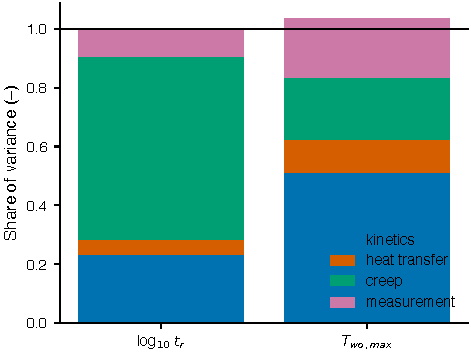
\includegraphics[width=0.6\textwidth]{fig15_variance_shares}
\caption{One-group-at-a-time shares of the variance of $\log_{10} t_r$ and of the hot-spot temperature at the S1 base point; numerical values in Table~\ref{tab:variance}.}
\label{fig:shares}
\end{figure}


The one-group-at-a-time shares sum to unity within 0.04, so the four groups act almost additively and the interaction between them is negligible at the base point. The share of the creep group in the hot-spot temperature (0.211) is not a feedback of the creep model on the thermal solution, which does not exist, but the effect of the wall thickness, which belongs to the creep group because it also enters the hoop stress and which changes the conduction drop across the tube wall.

% =====================================================================
\section{Supplementary figures}
\label{sec:figures}

\begin{figure}[h]
\centering
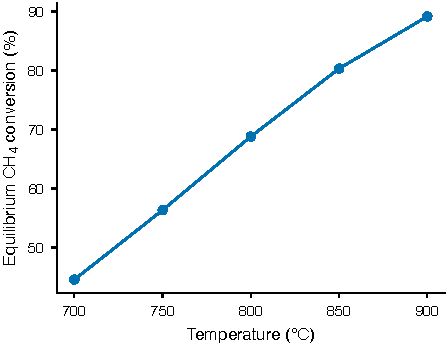
\includegraphics[width=0.75\textwidth]{fig00_equilibrium_conversion}
\caption{Equilibrium methane conversion of a CH$_4$/H$_2$O mixture at 25~bar and a steam-to-carbon ratio of 3, computed with Cantera and the GRI-Mech~3.0 thermodynamic data. This is the thermodynamic ceiling against which the reactor model is checked; at 850~$^\circ$C the equilibrium conversion is 0.80 and the dry hydrogen fraction 73\,\%.}
\label{fig:equilibrium}
\end{figure}

\begin{figure}[h]
\centering
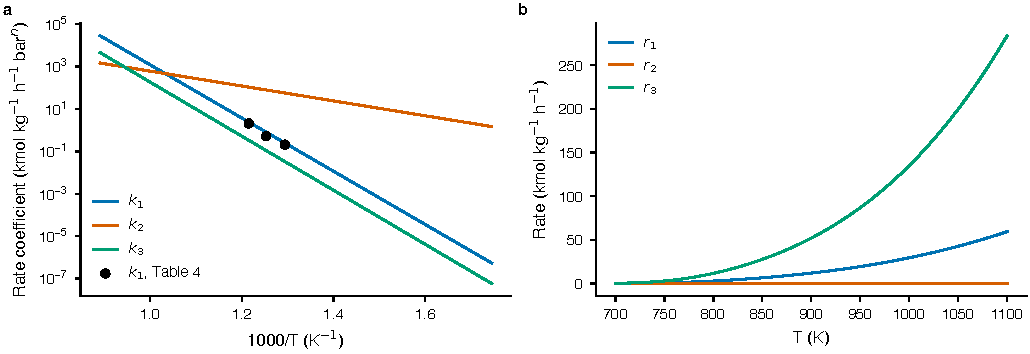
\includegraphics[width=\textwidth]{fig01_kinetics}
\caption{Xu--Froment kinetics as implemented: (a) Arrhenius plot of the rate coefficients $k_1$, $k_2$ and $k_3$ against $1000/T$, with the per-temperature estimates of Table~4 of~\cite{xu1989a} overlaid, and (b) the three reaction rates against temperature at 25~bar for a CH$_4$:H$_2$O:H$_2$ feed of 1:3:0.1.}
\label{fig:kinetics}
\end{figure}

\begin{figure}[h]
\centering
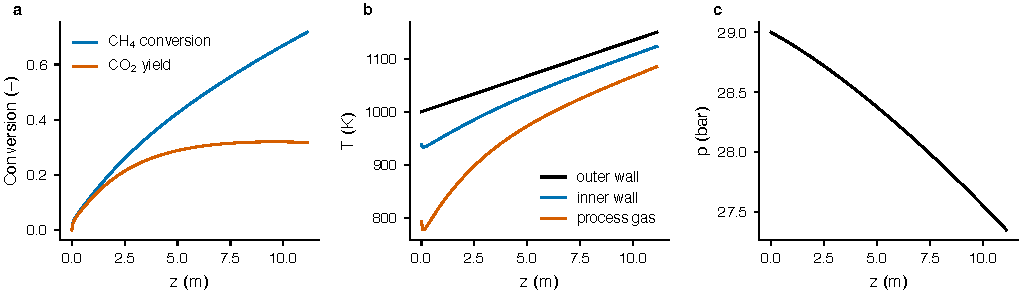
\includegraphics[width=\textwidth]{fig02_reactor_profiles}
\caption{Stand-alone tube model with a prescribed linear outer-wall profile: (a) methane conversion and CO$_2$ yield, (b) process-gas, inner-wall and outer-wall temperatures and (c) pressure along the tube for the feed of Table~2 of~\cite{xu1989b}. This run precedes the verification of the main text and uses no fitted parameters.}
\label{fig:profiles}
\end{figure}

\begin{figure}[h]
\centering
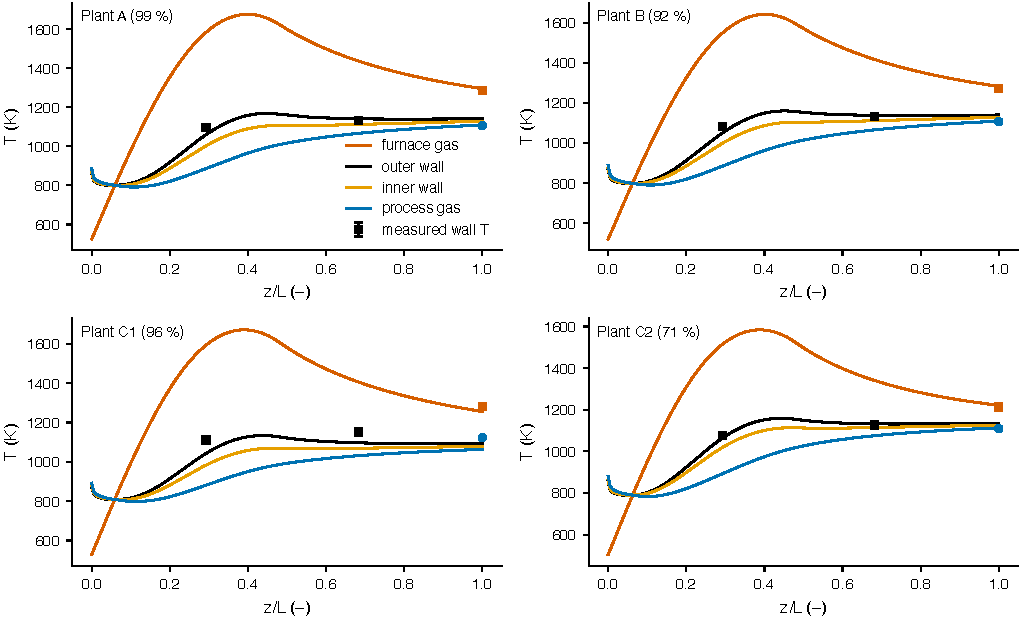
\includegraphics[width=\textwidth]{fig04_latham_baseline}
\caption{Coupled furnace--tube model before calibration, with the parameter values of Table~6 of~\cite{latham2011} transferred directly: axial temperature profiles for the plant cases and the measured wall temperatures. Three of the four cases are reproduced within the measurement uncertainty without any fitting.}
\label{fig:baseline}
\end{figure}

\begin{figure}[h]
\centering
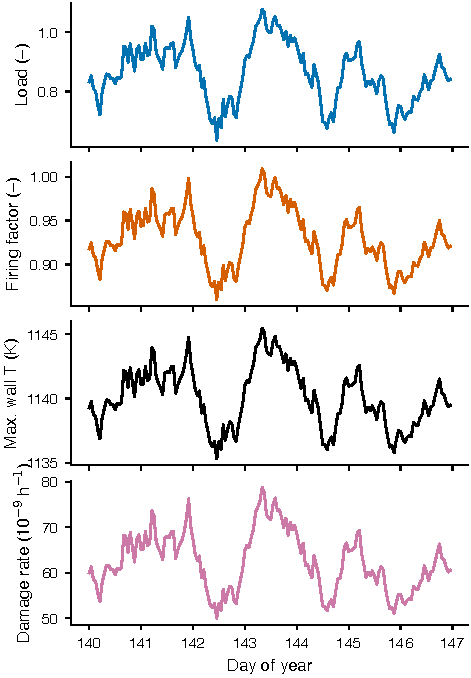
\includegraphics[width=\textwidth]{fig10_scenarios_timeseries}
\caption{One representative week of the renewable-following scenario S3: load, firing factor, hot-spot temperature and hourly damage rate. The damage rate follows the hot spot through the Larson--Miller relation and is therefore strongly non-linear in the load.}
\label{fig:timeseries}
\end{figure}

\begin{thebibliography}{99}
\bibitem{xu1989a} J. Xu, G.~F. Froment, Methane steam reforming, methanation and water-gas shift: I. Intrinsic kinetics, AIChE J. 35 (1989) 88--96.
\bibitem{xu1989b} J. Xu, G.~F. Froment, Methane steam reforming: II. Diffusional limitations and reactor simulation, AIChE J. 35 (1989) 97--103.
\bibitem{latham2011} D.~A. Latham, K.~B. McAuley, B.~A. Peppley, T.~M. Raybold, Mathematical modeling of an industrial steam-methane reformer for on-line deployment, Fuel Process. Technol. 92 (2011) 1574--1586.
\bibitem{wesenberg2007} M.~H. Wesenberg, H.~F. Svendsen, Mass and heat transfer limitations in a heterogeneous model of a gas-heated steam reformer, Ind. Eng. Chem. Res. 46 (2007) 667--676.
\bibitem{hawthorne1949} W.~R. Hawthorne, D.~S. Weddell, H.~C. Hottel, Mixing and combustion in turbulent gas jets, Third Symposium on Combustion and Flame and Explosion Phenomena 3 (1949) 266--288.
\bibitem{sklearn} F. Pedregosa, G. Varoquaux, A. Gramfort, V. Michel, B. Thirion, O. Grisel, M. Blondel, P. Prettenhofer, R. Weiss, V. Dubourg, J. Vanderplas, A. Passos, D. Cournapeau, M. Brucher, M. Perrot, \'E. Duchesnay, Scikit-learn: machine learning in Python, J. Mach. Learn. Res. 12 (2011) 2825--2830.
\bibitem{yeh2021} C.-L. Yeh, Numerical analysis of the combustion and transport phenomena in a reformer tube, Appl. Sci. 11 (2021) 231.
\end{thebibliography}

\end{document}